\documentclass[10pt,twocolumn]{article}
\usepackage[margin=0.75in]{geometry}
\usepackage{amsmath,amssymb}
\usepackage{graphicx}
\usepackage{array}
\usepackage{booktabs}
\usepackage{times}
\usepackage[hidelinks]{hyperref}

\setlength{\parindent}{1em}
\setlength{\parskip}{2pt}
\newcommand{\Rcomf}{R_{\mathrm{comf}}}
\newcommand{\Rcc}{R_{\mathrm{cc}}}

\title{\textbf{One Policy for the Whole Arm: Region-Conditioned Distillation\\
for Safe Robotic Bed-Bathing}}
\author{Authors: TBD \\ \textit{Draft --- ICRA submission}}
\date{}

\begin{document}
\maketitle

\begin{abstract}
Robotic assistance with bed-bathing requires a manipulator to wipe the skin of a supine
person completely, systematically, and with clinically safe contact forces. Reinforcement
learning (RL) can produce competent per-region wiping policies, but deploying a separate
network for every body part is impractical, and the standard contact-counting reward
optimizes the wrong objective---it clears targets aggressively without regard to coverage or
force safety. We make three contributions. First, the \emph{Comfort reward}: a structured
wiping reward that shapes motion along a self-supervised arm axis---extended here with a 2-D
(length\,$\times$\,circumference) coverage term built from the same SVD's second principal
axis---producing complete, force-safe sweeps. Second, a \emph{single distilled policy
conditioned on region and a one-bit comfort dial} that replaces eight per-region specialists,
matches or exceeds them in every region, and beats a flat multi-task policy by \textbf{+33\%
targets cleared (positive in 12/12 region$\times$seed pairs, exact sign test $p=0.0005$)} while
keeping contact force in the therapeutic band 2--2.7$\times$ more often. Third, the dial bit
exposes a \emph{caregiver-selectable gentle$\leftrightarrow$thorough} behavior: in a paired
same-network test, the Comfort-reward (Gentle) setting raises therapeutic-band adherence by
\textbf{+34\% (10/12 pairs, $p=0.039$)} at an 8\% coverage cost. Across the full method ladder,
learning dominates a scripted geometric controller on every wiping-quality metric---the
scripted sweep traces near-perfect geometry yet fails sustained safe contact---and the reward
design decides not how \emph{much} the robot wipes but how \emph{safely}.
\end{abstract}

\section{Introduction and Problem Definition}
A UR5 manipulator holds a soft tool and cleans a target region of a supine human arm in
simulation (PyBullet). Each region carries up to 15 cleanable \emph{targets}; a target is
\emph{cleared} when the tool passes within $\texttt{clear\_radius}=0.022$\,m while in contact.
Episodes last 150 steps. The observation is a 90-D vector (robot joint state, end-effector
pose, tool--skin contact geometry, region/target encoding); the action is a 6-D continuous
end-effector command.

\textbf{Why raw clear-count is the wrong objective.} Assistive bathing is a
\emph{coverage-and-safety} task, not a target-collection game. A caregiver wipes the whole
region in order, maintaining gentle, sustained skin contact. A reward that simply counts
contacts encourages fast, aggressive dabbing that inflates the clear-count while leaving gaps
and spiking force. We therefore evaluate on a battery of behavior metrics (Sec.~\ref{sec:metrics})
and design a reward---the \emph{Comfort reward}---for the true objective.

\textbf{Why one policy, not four.} Region-specialist policies are easy to train but
impractical to deploy: a robot would need to store and select among a library of networks. We
ask whether a \emph{single} context-conditioned policy, distilled from the specialists, can
replace the whole library without loss---the paper's central generalization question.

\section{Method}
\subsection{Teacher policies}
One PPO policy (RLlib 1.13) per (region, reward) pair. Policy/value net
$\texttt{fcnet\_hiddens}=[100,100]$, tanh; $\texttt{train\_batch\_size}=19200$,
$\texttt{num\_sgd\_iter}=50$, $\texttt{sgd\_minibatch\_size}=128$. Trained in $\sim$250k-step
chunks with best-checkpoint archiving.

\subsection{Reward design}
\label{sec:reward}
We compare two reward designs on identical dynamics. The baseline is the naive
contact-counter; the proposed \emph{Comfort reward} keeps its base terms and adds
coverage-and-safety shaping.

\textbf{Baseline: Contact-count reward $\Rcc$.} The original reward shipped with the public
bed-bathing codebase (git \texttt{96fb9af}):
\begin{equation}
\Rcc = w_d\,(-d_{\text{arm}}) + w_a\,(-\lVert a\rVert^2) + w_c\,c_t,
\label{eq:cc}
\end{equation}
with $(w_d,w_a,w_c)=(1.0,\,0.01,\,5.0)$, where $d_{\text{arm}}$ is tool--arm distance, $a$ the
action, and $c_t$ the targets cleared at step $t$. It rewards \emph{how many} targets are
cleared but has no notion of \emph{where} along the arm the tool is or whether coverage is
systematic.

\textbf{Proposed: Comfort reward $\Rcomf$.} We keep the base terms and add four
coverage-shaping terms:
\begin{align}
\Rcomf &= w_d\,r_{\text{dist}} + w_a\,r_{\text{act}} + w_c\,r_{\text{clr}}
   \nonumber\\
   &\quad + w_s\,r_{\text{sweep}} + w_w\,r_{\text{win}} + w_e\,r_{\text{end}}
        + w_v\,r_{\text{cov}},
\label{eq:comf}
\end{align}
with weights $(w_d,w_a,w_c,w_s,w_w,w_e,w_v)=(1.0,\,0.01,\,5.0,\,1.0,\,1.0,\,1.0,\,1.0)$,
$r_{\text{act}}=-\lVert a\rVert^2$, and $r_{\text{clr}}=c_t$. Table~\ref{tab:reward}
summarizes each term; the four shaping terms are detailed below.

\emph{Two-phase distance ($r_{\text{dist}}$).} $r_{\text{dist}}=-d_{\text{arm}}$ while
reaching, switching to the along-surface distance once wiping, so the policy is rewarded for
staying on-surface rather than merely approaching.

\emph{Self-supervised sweep axis ($r_{\text{sweep}}$).} Let $u$ be the principal axis of the
target cloud (SVD, refreshed every $\sim$200 steps) and $p$ the tool position. The normalized
sweep coordinate is
$s=\mathrm{clip}\!\big((\langle p-\bar p,\,u\rangle - s_{\min})/\mathrm{span},\,0,\,1\big)$.
With $\Delta s_{\text{dir}} = \rho\,(s_t-s_{t-1})$ for pass direction $\rho\in\{\pm1\}$,
\begin{equation}
r_{\text{sweep}}=
\begin{cases}
k_f \min(\Delta s_{\text{dir}},\delta), & \Delta s_{\text{dir}} > \varepsilon\\[2pt]
-k_b \min(-\Delta s_{\text{dir}},\delta), & \Delta s_{\text{dir}} < -\varepsilon\\[2pt]
0, & \text{otherwise,}
\end{cases}
\end{equation}
active only while in contact ($k_f{=}0.5,k_b{=}0.75,\varepsilon{=}0.01,\delta{=}0.05$). It
rewards monotone progress along the arm and mildly penalizes backtracking.

\emph{Local window ($r_{\text{win}}$).} $r_{\text{win}}=0.5\,n^{\text{win}}_{\text{contact}}
+0.25\,n^{\text{win}}_{\text{clr}}$, crediting contact/clears near the current $s$
(discourages teleporting between distant targets).

\emph{Evidence-gated end-of-pass bonus ($r_{\text{end}}$).} $r_{\text{end}}=B$ ($B{=}4.0$)
when a pass reaches an end ($s\!\ge\!0.90$ forward or $s\!\le\!0.10$ backward) \emph{and} the
pass accumulated real coverage evidence ($\ge 1$ in-window hit/clear); otherwise $0$. The gate
prevents farming the bonus by sweeping empty space. A soft-contact latch with hysteresis
(6 steps) stabilizes the wipe/exit phase against brief force dropouts.

\emph{2-D $(s,w)$ coverage ($r_{\text{cov}}$).} For this elongated target geometry the
\emph{second} principal axis of the same SVD is the circumferential (``column'') direction;
projecting the tool onto it yields a normalized width coordinate $w\in[0,1]$. The first
contact or clear in each unvisited cell of a $4\times4$ $(s,w)$ grid earns
$r_{\text{cov}}=1$ once per episode ($w_v{=}1.0$ selected by grid search over
$\{0,0.5,1,2\}$: 6.08 vs.\ 5.68 targets cleared at $w_v{=}0$). The 1-D sweep terms reward
progress \emph{along} the arm only; this term is what gives the policy an incentive to cover
\emph{across} it.

\begin{table}[t]
\centering\small
\begin{tabular}{llc}
\toprule
\textbf{Term} & \textbf{What it rewards} & \textbf{Weight}\\
\midrule
$r_{\text{dist}}$  & on-surface proximity (two-phase) & $1.0$\\
$r_{\text{act}}$   & $-\lVert a\rVert^2$ (effort penalty) & $0.01$\\
$r_{\text{clr}}$   & targets cleared this step $c_t$ & $5.0$\\
$r_{\text{sweep}}$ & monotone progress along arm axis & $1.0$\\
$r_{\text{win}}$   & contact/clears near current $s$ & $1.0$\\
$r_{\text{end}}$   & evidence-gated end-of-pass bonus & $1.0$\\
$r_{\text{cov}}$   & first visit to each $(s,w)$ grid cell & $1.0$\\
\bottomrule
\end{tabular}
\caption{Terms of the Comfort reward $\Rcomf$ (Eq.~\ref{eq:comf}). The Contact-count baseline
$\Rcc$ (Eq.~\ref{eq:cc}) uses only the first three rows. The four shaping terms turn a
target-collector into a systematic, force-safe wiper.}
\label{tab:reward}
\end{table}

\subsection{Region-conditioned student}
A single Gaussian MLP policy conditioned on the region:
\begin{align*}
\text{input} &= [\, \text{obs}(90),\ \text{context}\,] \\
\text{context} &= \text{region one-hot}(4)\ [\,+\ \text{dial bit}(1)\,] \\
\text{backbone} &= \text{MLP}(128,128),\ \tanh \\
\text{heads} &= \text{mean}(6);\ \ \log\text{-}\mathrm{std}(6)\in[-5,2]
\end{align*}
a diagonal Gaussian $\pi_\theta(a\mid o,c)=\mathcal{N}(\mu_\theta,\,\mathrm{diag}\,\sigma_\theta^2)$.
At deployment the one-hot selects the current body part and the optional \emph{comfort dial}
bit $\kappa\in\{0,1\}$ selects behavior; one network covers the whole arm.

\subsection{Distillation}
\label{sec:distill}
Each teacher $\pi_r$ is rolled out in its own region to record
$(o,\ \mu_r(o),\ \log\sigma_r(o),\ c(r))$, i.e.\ the observation, the teacher's
diagonal-Gaussian action mean and log-std, and its context vector. Pooling all regions gives
$\mathcal{D}=\bigcup_r\mathcal{D}_r$. The student $\pi_\theta$ is fit by supervised
distillation---a behavior-cloning term on the mean plus a distribution-matching term on the
full Gaussian:
\begin{equation}
L(\theta)=\underbrace{\lVert \mu_\theta-\mu_T\rVert^2}_{\text{behavior clone}}
 +\ \beta\,\underbrace{\mathrm{KL}\!\big(\mathcal{N}_T\,\big\|\,\mathcal{N}_\theta\big)}_{\text{uncertainty match}},
\label{eq:loss}
\end{equation}
where, for diagonal Gaussians with per-dimension means $\mu$ and log-stds $\ell=\log\sigma$,
\begin{equation}
\begin{aligned}
\mathrm{KL}\!\big(\mathcal{N}_T\,\|\,\mathcal{N}_\theta\big)=
\sum_{i=1}^{6}\Big[\,&\ell_{\theta,i}-\ell_{T,i}-\tfrac12\\[-1pt]
&+\frac{\sigma_{T,i}^2+(\mu_{T,i}-\mu_{\theta,i})^2}{2\,\sigma_{\theta,i}^2}\Big].
\end{aligned}
\label{eq:kl}
\end{equation}
We minimize the batch mean of Eq.~\ref{eq:loss} with Adam (lr $10^{-3}$, $\beta{=}1$),
matching both the teacher's action mean and its uncertainty. We compare four distillation
sources: \textbf{Comfort} (4 Comfort-reward teachers), \textbf{Contact-count} (4
contact-counting teachers), \textbf{dial-conditioned} (all 8 teachers $+$ a comfort-dial bit
that switches behavior on demand), and \textbf{flat} (all 8 pooled, no bit---an irreversible
blend).

\vspace{2pt}
\noindent\fbox{\parbox{0.95\columnwidth}{
\footnotesize
\textbf{Algorithm 1: Region-conditioned distillation}\\[2pt]
\textbf{Input:} teachers $\{\pi_r\}_{r\in R}$; context map $c(r)$; rollout length $N$;
weight $\beta$; (optional) dial values $\{\kappa_r\}$.\\
1. \textbf{Collect:} for each region $r$, roll out $\pi_r$ for $N$ steps; record
$(o,\ \mu_r(o),\ \log\sigma_r(o),\ c(r))$ where $\mu_r,\log\sigma_r$ are the teacher's
DiagGaussian parameters. Append dial bit $\kappa_r$ to $c(r)$ if given.\\
2. \textbf{Pool:} $\mathcal{D}=\bigcup_r \mathcal{D}_r$.\\
3. \textbf{Train} $\pi_\theta(a\,|\,o,c)$ by minibatch Adam ($10^{-3}$) on the mean of
Eq.~\ref{eq:loss} (BC $+\,\beta\,$KL, Eq.~\ref{eq:kl}).\\
\textbf{Output:} single conditioned student $\pi_\theta$.
}}

\section{Experimental Design}
\textbf{Regions (4):} forearm back/front, upper-arm back/front.

\subsection{Methods and baselines}
We evaluate three reward classes---Comfort RL, Contact-count RL, and a non-RL scripted
geometric sweep---each as \emph{both} a per-region specialist \emph{and} a distilled student,
plus:
\begin{itemize}\itemsep1pt
\item \textbf{Dial student (proposed)}: \emph{one} policy distilled from all eight RL
specialists, conditioned on region and a one-bit comfort dial; evaluated at both dial ends,
\emph{Gentle} ($\kappa{=}0$, Comfort behavior) and \emph{Thorough} ($\kappa{=}1$,
Contact-count behavior).
\item \textbf{Comfort / Contact-count specialists / students}: per-region PPO teachers and
their single-family region-conditioned distilled students.
\item \textbf{Scripted specialist / student}: the geometric sweep, and a student
behavior-cloned from it (does a non-RL controller generalize when cloned?).
\item \textbf{Flat baseline}: a \emph{single} PPO policy trained jointly on all four regions
with the Comfort reward and \emph{no} region conditioning---the direct multi-task alternative
to distillation.
\end{itemize}

\subsection{Evaluation protocol}
Every method is scored by identical reducers (\texttt{metrics\_report.episode\_metrics}),
200 episodes per region (100 for the deterministic scripted controller), force band
$[2,12]$\,N, $\texttt{clear\_radius}=0.022$\,m, and \textbf{3 training seeds} for every
learned method. For significance we use exact sign tests over the 12 region$\times$seed
pairs plus a conservative per-seed paired $t$-test---the seed, not the episode, is the
statistical unit (episode-level pooling would be pseudoreplication). Every number below is
emitted by \texttt{analyze\_final.py} from the raw metrics CSV.

\subsection{Evaluation metrics}
\label{sec:metrics}
Per step $t$ an episode yields normal force $f_t$, an in-contact flag, sweep coordinate
$s_t\in[0,1]$, per-step clears $k_t$, and action $a_t$; $\mathcal{C}=\{t:\text{contact}\}$
denotes the in-contact steps and $T$ the episode length. Table~\ref{tab:metrics} defines the
curated headline set with exact formulas.

\begin{table*}[t]
\centering\footnotesize
\setlength{\tabcolsep}{5pt}
\begin{tabular}{@{}p{0.19\textwidth} p{0.50\textwidth} p{0.26\textwidth}@{}}
\toprule
\textbf{Metric} & \textbf{Definition} & \textbf{What it captures}\\
\midrule
Targets cleared        & $\sum_t k_t$ \ (distinct, out of 15) & task performance\\
In-band force fraction & $\big|\{t\in\mathcal{C}:f_t\in[2,12]\,\text{N}\}\big|\,/\,|\mathcal{C}|$ & contact-force safety\\
Contact-time fraction  & $|\mathcal{C}|\,/\,T$ & sustained skin engagement\\
Sweep consistency      & (forward-progress wipe steps)$\,/\,$(wipe steps) & systematic, monotone motion\\
Clear $s$-coverage     & $\big|\{\text{arm-axis bins with a clear}\}\big|/B,\ B{=}10$ & spatial spread along the arm\\
Clear $t$-coverage     & $\big|\{\text{time bins with a clear}\}\big|/B,\ B{=}10$ & temporal spread (not bursty)\\
Second-half fraction   & $\big(\sum_{t>T/2}k_t\big)\big/\sum_t k_t$ & sustained, not front-loaded\\
Clear spatial order    & fraction of consecutive clears moving in the dominant $s$-direction & orderly sweep ($1.0$) vs.\ random ($0.5$)\\
Mean stroke length     & mean length of maximal in-contact, constant-direction sliding runs & wipe (long) vs.\ poke (short)\\
Contact bouts          & number of separate contact episodes & poking fragments contact (higher $=$ worse)\\
Slide fraction         & $\big|\{t\in\mathcal{C}:|\Delta s_t|>0.008\}\big|/|\mathcal{C}|$ & sliding vs.\ tapping in place\\
Peak force             & $\max_{t\in\mathcal{C}} f_t$ & worst-case contact force (lower is safer)\\
\bottomrule
\end{tabular}
\caption{Evaluation metrics with exact definitions. Two families are deliberately
\emph{excluded} from cross-method comparison. \emph{Pass completions} counts firings of the
Comfort reward's own end-of-pass gate, so it measures one method's internal machinery.
\emph{Mean/p95 force} reward \emph{not touching}---the scripted controller has the lowest mean
force precisely because it grazes---so force safety is reported as in-band fraction and peak
force only. Remaining metrics (task success, action effort/smoothness, stall fraction) are
retained in the appendix.}
\label{tab:metrics}
\end{table*}

\section{Results}

\begin{table*}[t]
\centering\small
\setlength{\tabcolsep}{3pt}
\begin{tabular}{lccccc}
\toprule
 & \multicolumn{5}{c}{\textbf{cleared\,/\,15\ \ (in-band force fraction), 3-seed mean}}\\
\cmidrule(l){2-6}
\textbf{Method} & \textbf{forearm back} & \textbf{forearm front} & \textbf{upper-arm back} & \textbf{upper-arm front} & \textbf{mean}\\
\midrule
Comfort specialist          & 6.25 (0.150) & 4.99 (0.218) & 6.75 (0.164) & 5.19 (0.159) & 5.80 (0.173)\\
Contact-count specialist    & 6.72 (0.121) & 7.05 (0.256) & 6.80 (0.112) & 4.95 (0.128) & 6.38 (0.154)\\
Student $\leftarrow$ Comfort       & 6.15 (0.154) & 6.23 (\textbf{0.282}) & 6.74 (0.172) & \textbf{5.96} (0.162) & 6.27 (\textbf{0.193})\\
Student $\leftarrow$ Contact-count & 6.42 (0.117) & 7.77 (0.256) & 6.82 (0.110) & 5.69 (0.128) & 6.68 (0.153)\\
Dial @Gentle                & 6.35 (0.168) & 6.15 (\textbf{0.311}) & 6.62 (0.165) & 5.55 (0.146) & 6.17 (\textbf{0.198})\\
Dial @Thorough              & \textbf{6.95} (0.121) & 7.65 (0.278) & \textbf{7.02} (0.106) & 5.56 (0.120) & \textbf{6.80} (0.156)\\
Flat (multi-task)           & 5.00 (0.073) & 5.20 (0.059) & 6.43 (0.109) & 3.80 (0.058) & 5.11 (0.075)\\
Scripted (non-RL)           & 6.27 (0.087) & 4.48 (0.050) & 4.28 (0.020) & 3.20 (0.002) & 4.56 (0.040)\\
\bottomrule
\end{tabular}
\caption{\textbf{Main comparison} across all four arm regions (3 seeds each). Each cell is
targets cleared out of 15 with the therapeutic-band (2--12\,N) force fraction in parentheses;
bold marks the best coverage (per region) and the best in-band fraction. The conditioned
students and the comfort dial dominate the flat multi-task and non-RL scripted baselines on
both coverage and in-band force; the dial's two ends bracket the
coverage$\leftrightarrow$gentleness trade-off. Numeric companion to Fig.~\ref{fig:matrix}.}
\label{tab:main}
\end{table*}

\subsection{Headline: one network with a caregiver-selectable gentle$\leftrightarrow$thorough dial}
The dial student---a single network conditioned on region and one comfort-dial bit---spans the
coverage$\leftrightarrow$gentleness trade-off at deployment time. Averaged over 4 regions
$\times$ 3 seeds: \textbf{Thorough mode 6.80 cleared / 0.156 in-band}, \textbf{Gentle mode
6.17 cleared / 0.198 in-band}, with the ordering consistent on all four regions
(Table~\ref{tab:dial}). At each end the dial matches or exceeds the corresponding
single-reward student---it is not a compromise but both behaviors in one deployable policy.
Table~\ref{tab:main} reports every method across all four arm regions.

\begin{table}[h]
\centering\small
\setlength{\tabcolsep}{4pt}
\begin{tabular}{lcc}
\toprule
\textbf{Region} & \textbf{Gentle} & \textbf{Thorough} \\
 & \textbf{\footnotesize clr / in-band} & \textbf{\footnotesize clr / in-band} \\
\midrule
forearm back    & 6.35 / \textbf{0.168} & \textbf{6.95} / 0.121 \\
forearm front   & 6.15 / \textbf{0.311} & \textbf{7.65} / 0.278 \\
upper-arm back  & 6.62 / \textbf{0.165} & \textbf{7.02} / 0.106 \\
upper-arm front & 5.55 / \textbf{0.146} & \textbf{5.56} / 0.120 \\
\bottomrule
\end{tabular}
\caption{The comfort dial per region (3-seed means): the Gentle end is gentler (higher
in-band) in 4/4 regions, the Thorough end clears $\geq$ in 4/4.}
\label{tab:dial}
\end{table}

\subsection{The distilled policy beats the flat multi-task baseline}
The dial in Thorough mode clears \textbf{6.80} vs \textbf{5.11} for the flat
baseline---\textbf{+33\%}, positive in \textbf{12/12 region$\times$seed pairs} (exact sign
test $p=0.0005$), consistent per seed ($6.43/6.81/7.14$ vs $5.26/5.37/4.69$). The
Comfort-distilled student alone gains $+1.16$ clears/seed (per-seed paired $t=3.76$, $n=3$;
10/12 pairs, sign $p=0.039$). Conditioning also buys \emph{safety}: every conditioned
student keeps force in-band 2--2.7$\times$ more than the flat baseline (0.153--0.198 vs
0.074). One network replaces four specialists and beats the unconditioned alternative on
both axes.

\subsection{Distillation $\geq$ specialists---and rescues weak teachers}
Students match their specialists where those are strong and repair them where they are weak
(cleared/15, 3-seed means): Comfort teacher$\to$student $4.99\to\textbf{6.23}$ on forearm
front and $5.19\to\textbf{5.96}$ on upper-arm front; Contact-count
$4.95\to\textbf{5.69}$ on upper-arm front. No region regresses by more than 0.3. Grand means:
students 6.17--6.80 vs specialists 5.79--6.38---pooled-data distillation regularizes.

\subsection{The reward style determines gentleness: a paired same-network test}
Because the dial student is \emph{one} network, flipping the bit is a perfectly paired
comparison---same weights, seeds, and regions; only the dial input differs. Switching to the
Gentle (Comfort) setting raises \textbf{in-band force fraction by +34\%} (better in 10/12
region$\times$seed pairs, exact sign test $\mathbf{p=0.039}$) at an 8\% coverage cost (3/12,
n.s.). On the composite \emph{safe clears} (cleared$\,\times\,$in-band) the Comfort-distilled
student leads by +28\% (8/12 pairs, suggestive). Raw clear-count ordering is reversed (the
Thorough/Contact-count setting clears more): the reward design does not make wiping more
\emph{productive}, it makes it \emph{safer}---and the dial exposes exactly that trade-off to
the caregiver.

\subsection{Learning and conditioning both matter: the method ladder}
Grand means over 4 regions $\times$ 3 seeds form a monotone ladder: non-RL scripted
\textbf{4.56} cleared / \textbf{0.039} in-band $<$ flat RL \textbf{5.11} / 0.074 $<$
specialists 5.79--6.38 / 0.15--0.17 $<$ distilled students \textbf{6.17--6.80} / 0.15--0.20.
The scripted controller is not merely less productive: it fails the wiping-\emph{quality}
battery---in contact only 25--41\% of steps (vs 51--74\% for the dial), in-band force
collapsing to 0.020/0.002 on the upper arm---while its near-perfect clear spatial order
(0.997) shows it traces textbook geometry. Raw clear-count and geometric orderliness are
mirages of wiping; sustained safe contact had to be learned. Crucially, \textbf{distillation
cannot repair it}: cloning the scripted controller into a student adds a little coverage
($4.56\to5.05$ grand mean) but leaves in-band force at $\sim$0.04, versus $\sim$0.19 for the
RL students. Distillation \emph{amplifies} what a teacher already does; it cannot inject safe
contact a teacher never had---so the generalization is a property of the learned behavior,
not of the distillation mechanism.

\begin{figure*}[t]
\centering
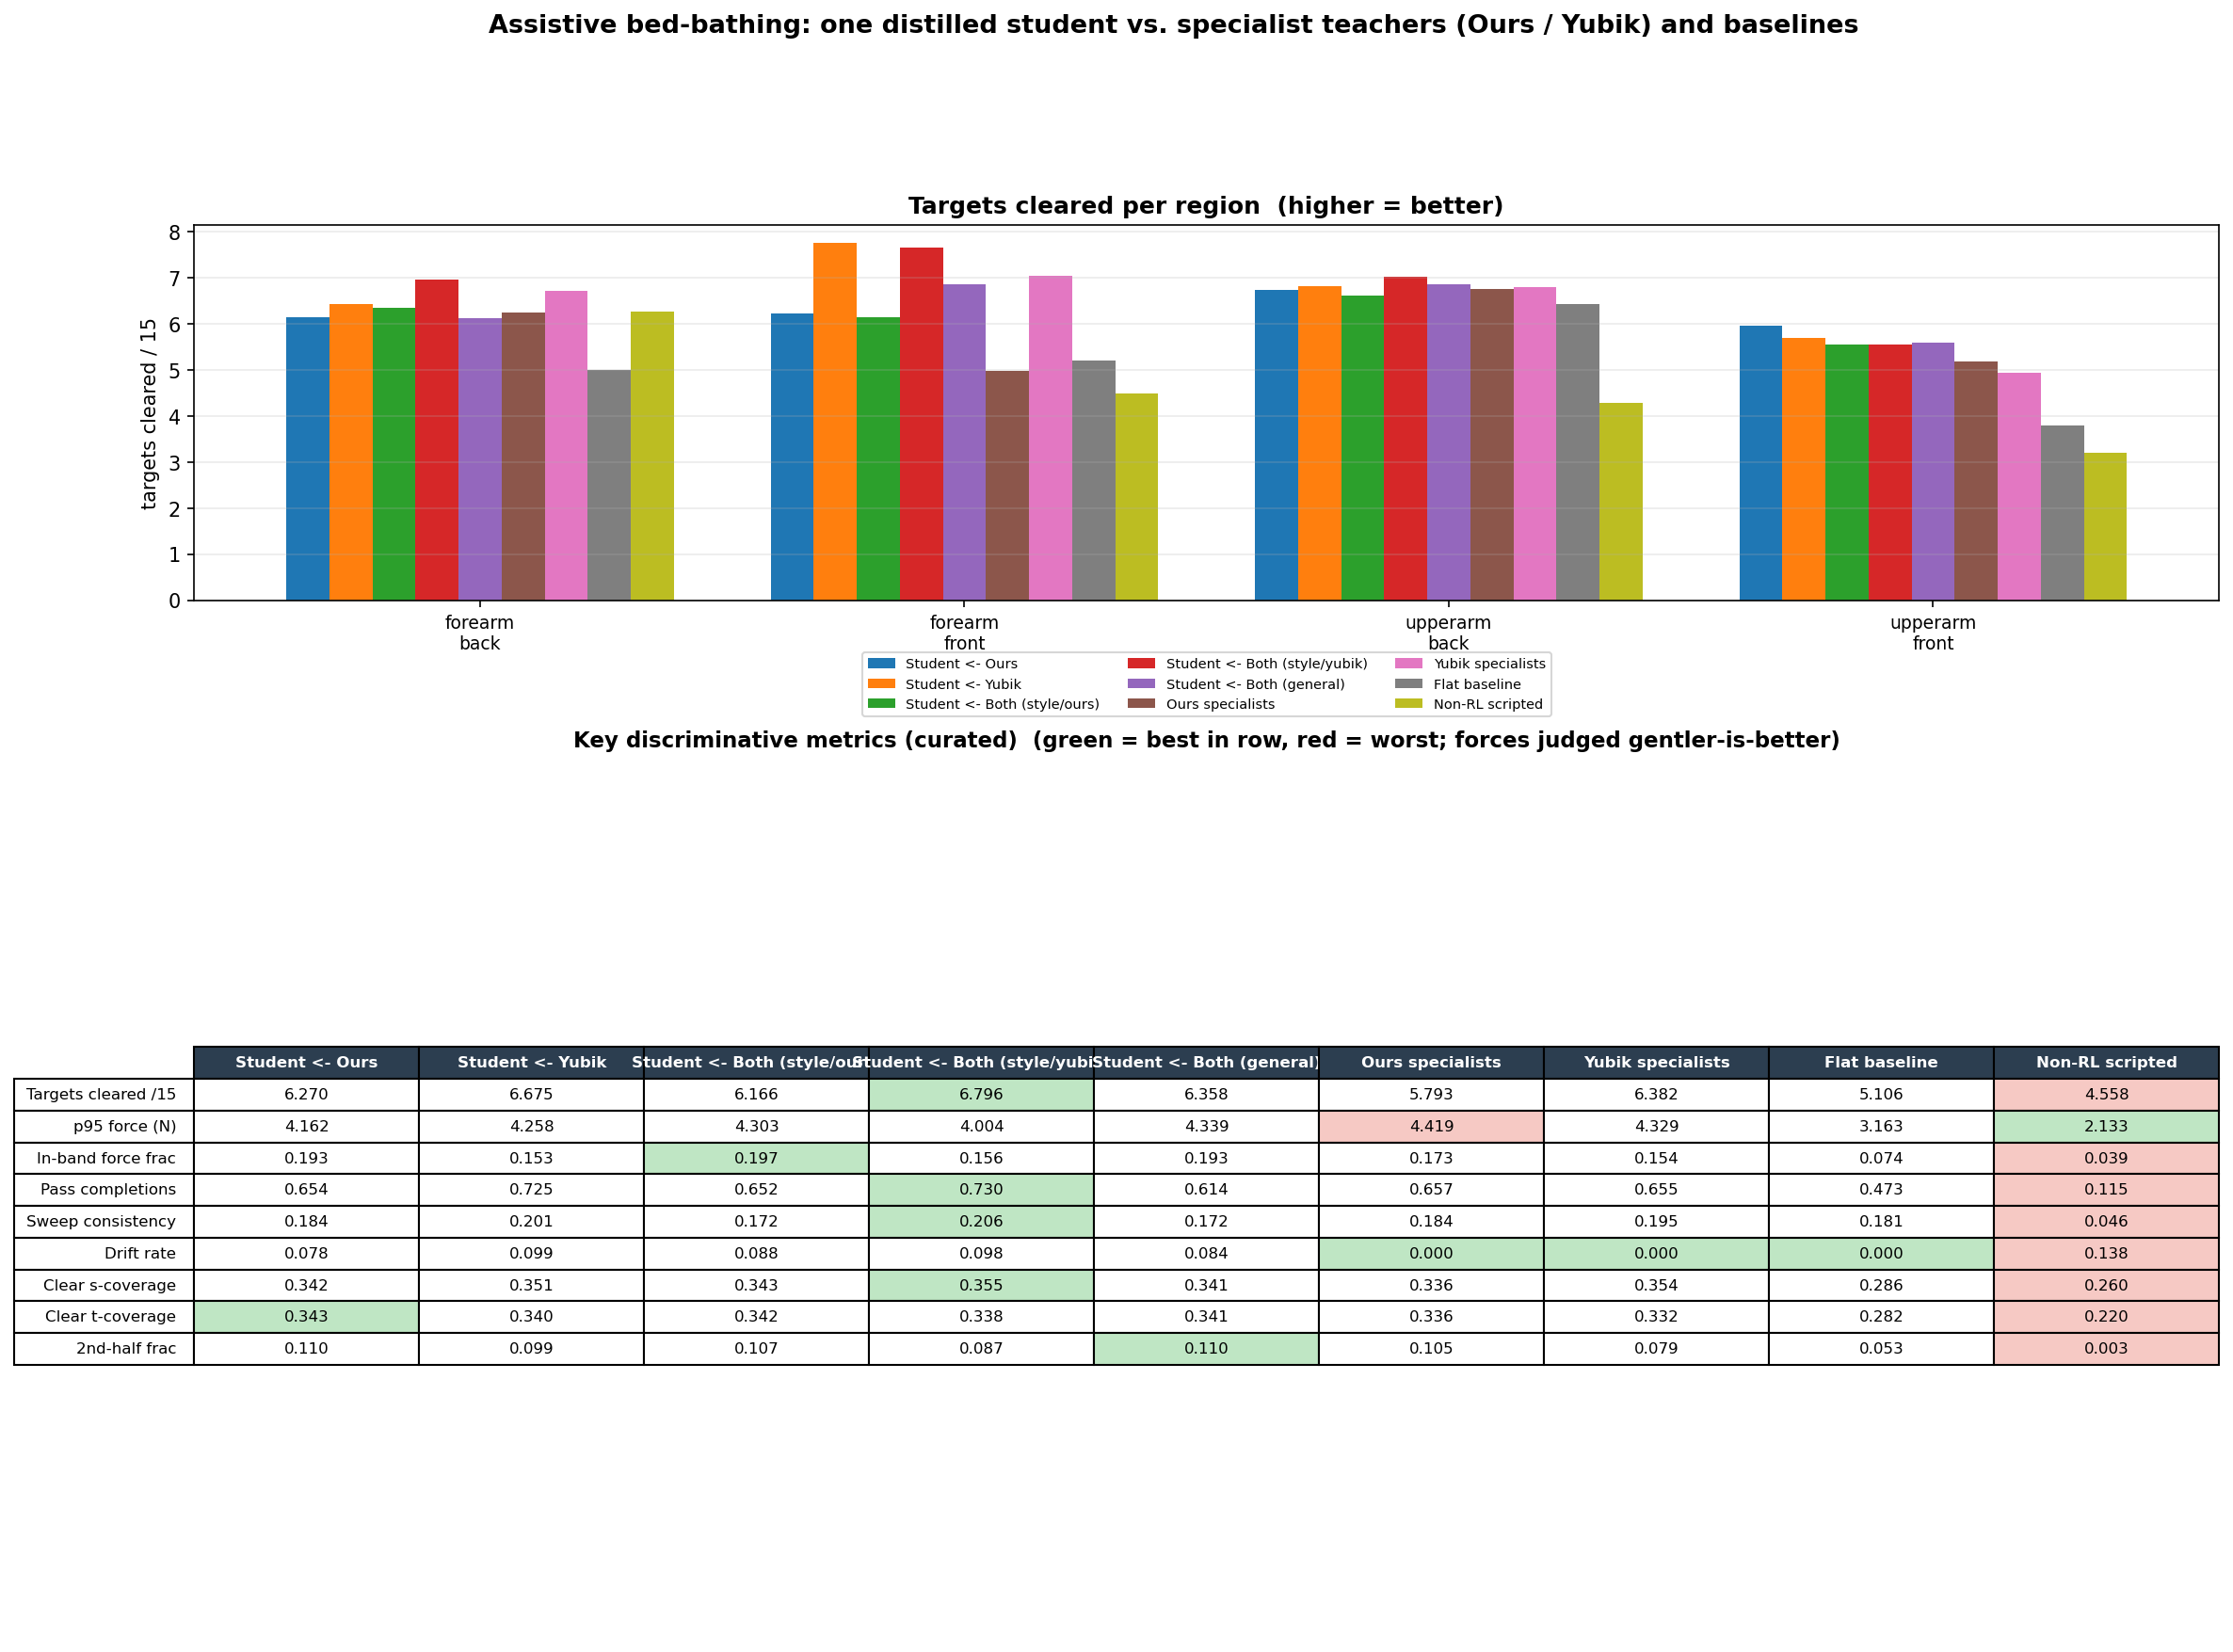
\includegraphics[width=0.98\textwidth]{ICRA_matrix_figure.png}
\caption{Method comparison across four arm regions and three seeds. Top: targets cleared per
region. Bottom: curated discriminative metrics (green = best in row, red = worst).}
\label{fig:matrix}
\end{figure*}

\section{Limitations}
\textbf{Reachability.} One angular column of each \emph{back} region faces the bed---the
supine limb's support surface. Per-target IK over a dense orientation grid, dynamic
clearability under three independent controllers, robot base-pose sweeps, and arm-posture
sweeps all show no configuration of this environment can wipe it (the humanoid lacks a
forearm pronation DOF). This caps targets-cleared near 10/15 on back regions and keeps
\texttt{task\_success} (69\% threshold) near zero for \emph{all} methods; cleaning the
support-facing surface requires physically re-positioning the limb---a caregiver action our
deployment pipeline assigns to its classical phases. \textbf{Force spikes.} Peak contact
forces reach 47--68\,N for all methods; bounding worst-case force (force-rate shaping or a
controller-level clamp) is required before hardware trials. \textbf{Statistics.} Sign tests
over 12 region$\times$seed pairs are exact, but per-seed $n=3$; per-method gaps quoted
without a $p$-value are directional. \textbf{Scope.} Results are simulation-only (rigid
humanoid, quasi-static scene); sim-to-real transfer is future work.

\section{Conclusion}
A single distilled policy, conditioned on region and a one-bit comfort dial, wipes all four
arm regions, beats the flat multi-task baseline in every region$\times$seed pair (+33\%,
$p=0.0005$), and exposes a caregiver-selectable gentle$\leftrightarrow$thorough behavior whose
Gentle end raises therapeutic-band adherence by 34\% in a paired same-network test
($p=0.039$). Across the method ladder, learning dominates scripting on every wiping-quality
metric, and conditioned distillation dominates flat multi-task RL on both coverage and
safety. The Comfort reward does not decide how \emph{much} a robot wipes---it decides how
\emph{safely}; distillation turns that choice into a runtime-switchable property of one
deployable network.

\end{document}
